\subsection{La développement}
Une fois la recherche bibliographique à peu près terminé, nous avons une idée plus clair de à quoi le simulateur devrait ressembler. Nous présenterons dans cette partie les différentes tâches effectués lors du développement du simulateur.
\emph{TODO: GANT}

\subsubsection{Le choix des outils}
Pour le développement de ce simulateur j'ai décidé d'utiliser le langage \gls{java}. En effet, j'avais déjà une expérience sur ce langage qui à été consolidé par l'enseignement reçu en DUT. \gls{java} est également plateforme ce qui permet au simulateur de pouvoir fonctionner sous la plupart des systèmes d'exploitation.\\

Pour ma gestion des librairies j'ai utilisé la technologie \gls{maven} qui permet de gérer très facilement ses librairies ainsi que la compilation des projets Java. Même si il peut y a voir quelques fois des complications, cet outils est généralement très facile d'utilisation.\\

J'ai décidé d'utiliser pour l'interface utilisateur la technologie \gls{javafx} qui est désormais intégré dans l'installation par défaut de Java. J'avais découvert cette technologie via mes camarades de promotions et l'est utilisé pour la première fois dans le projet de groupe du cours de \emph{CPOA} où nous avions réaliser une application de gestion d'un tournois de tennis. Le choix de cette technologie est logique au vu de sa puissance et sa facilité d'utilisation en comparaison des technologies plus anciennes comme \emph{AWT} ou \emph{Swing}.\\
Cependant, je n'étais pas totalement satisfait du rendu graphique de JavaFX, c'est pour cela que j'ai cherché une alternative qui me permette d'embellir mes interface graphiques. C'est alors que j'ai découvert la librairie \emph{JFoenix} qui implémente le Matérial Design, qui est un courant de design graphique numérique initié par Google, en JavaFX.

\subsubsection{L'architecture générale}
Avant de développer chaque fonctionnalité du simulateur il faut tout d'abord réfléchir à comment va s'organiser le code source. Le simulateur va prendre la forme d'une succession d'écrans dans lesquelles l'utilisateur pourra saisir des valeurs, une fois les valeurs vérifiés, l'utilisateur pourra passer à l'écran suivant. Une fois qu'un écran est complété, l'utilisateur peut revenir en arrière sur un autre écran afin de modifier ses valeurs.\\

Pour arriver à ce résultat, j'ai mis en pratique une notion que nous avons appris en DUT : le modèle MVC.
\begin{figure}[h]
	\begin{center}
		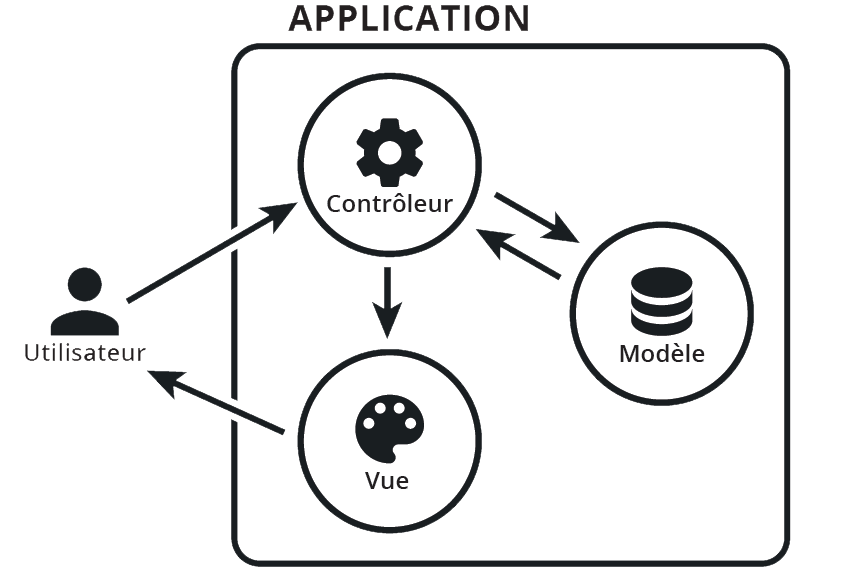
\includegraphics[scale=0.70]{partie2/images/mvc.png}
		\caption{Schéma du modèle MVC}
	\end{center}
\end{figure}

Le modèle MVC (Modèle-vue-contrôleur) est un modèle d'architecture logiciel destiné aux interfaces graphiques. Il se découpe en 3 modules effectuant chacun une action spécifique :
\begin{itemize}
	\item Le modèle qui s'occupe de récupérer les données à afficher dynamiquement,
	\item La vue qui contient toutes les composants graphiques,
	\item Le contrôleur qui s'occupe de récupérer et traiter les actions faites par l'utilisateur.\\
\end{itemize}

Ainsi chaque écran possède une vue et un contrôleur qui parfois va chercher des information dans un modèle. La vue est stocké sous forme de fichier FXML, qui est une implémentation du langage de balisage XML propre à JavaFX et qui nous permet de construire des vue à la manière d'une page web. Chaque vue, en plus des éléments graphiques, possède un nom, un numéro d'apparition ainsi qu'une référence vers leur contrôleur associé.
Afin de charger toutes les vues en mémoire le plus facilement possible, on les stocke dans un même dossier, ainsi au lancement du simulateur il suffira de récupérer la liste des fichiers de ce dossier, de lire le FXML de chaque fichier afin de créer la vue et d'y associer le contrôleur associé grâce à la référence stockée dans le fichier.

\subsubsection{L'architecture des contrôleurs}
Pour que le simulateur soit fonctionnel j'ai besoin d'effectuer certaines actions à certains moments dans l'exécution du programme. Je dois par exemple initialiser les composants graphiques de la vue une seule fois au tout début du programme pour qu'ils soient fonctionnel. J'ai également besoin, parfois d'effectuer des actions à chaque fois que l'utilisateur va sur un écran. Je dois également pouvoir être capable de changer les lignes de textes lorsque l'utilisateur demande à changer de langue.\\
Pour ce faire j'ai créé un \emph{interface} Java appelé \code{ViewController}, il s'agit d'une sorte de modèle que je peux appliquer à mes contrôleur afin qu'ils implémentent les modules que j'ai définis dans l'interface. Cet interface comporte donc 3 modules :
\begin{itemize}
	\item L'initialisation, qui s'exécute une seule fois par exécution du simulateur, au chargement de la vue en mémoire,
	\item Le chargement, qui s'exécute à chaque fois que l'utilisateur change d'écran,
	\item L'application de la langue, qui s'exécute à lorsque l'utilisateur souhaite changer la langue.
\end{itemize}
Ces trois modules étant essentiels pour chaque écran, tous mes contrôleur de vue implémentent cet interface.\\

J'ai également créé un autre interface Java, appelé \code{FormViewController}, qui lui ne sera appliqué qu'aux vues qui comporte un formulaire car il permet en implémentant les 3 modules suivant de gérer les champs des formulaire :
\begin{itemize}
	\item La sauvegarde, qui vérifie si les champs sont valides et lance la sauvegarde
	\item Le remplissage des champs, qui s'exécute lorsque l'on charge un sauvegarde en entrant les valeurs lues
	\item Le nettoyage des champs, qui supprime toutes les valeurs contenus dans les champs
\end{itemize} 

\subsubsection{La notion de simulation}
Pour que l'utilisateur puisse gérer facilement ses différentes configuration de centre de données qu'il rentre dans le simulateur j'ai décidé d'avancer la notion de simulation. Une simulation est tout simplement une instance du simulateur, elle contient un nom, des auteurs ainsi que tous les paramètres entrés par l'utilisateur durant l'exécution du programme. Cette simulation peut être facilement stocké et lue depuis le disque dur de l'utilisateur.\\

D'un point de vue technique, la simulation représente un objet Java que nous sérialisons au format JSON afin de la stocker sur le disque. Il nous suffira ensuite de la dé-sérialiser pour la charger en mémoire. J'ai fais le choix du format JSON car il est facilement lisible par l'humain et qu'il est extrêmement utilisé par les développeurs, la plupart des langages proposent des librairie pour le lire. Ainsi les fichiers de sauvegarde du simulateur pourrons facilement être utilisé dans d'autres programmes, même si ils ne sont pas développés en Java.\\

\subsubsection{La gestion de la langue}
Le laboratoire étant international j'ai naturellement penser à implémenter la possibilité de changer la langue du simulateur. Pour ce faire chaque ligne de texte qui est affichée à l'écran est codé par un identifiant unique. Par exemple l'identifiant \code{OPEN\_SIMULATION} représente la phrase \og Ouvrir une simulation \fg{} en français et la phrase \og Open a simulation \fg{} en anglais. Toutes les lignes de textes sont ainsi associé à leur identifiant dans un fichier de langue (que l'on appelle locale) situé dans un dossier de ressource. Chaque fichier contient également le nom de la langue, il nous suffit alors, comme pour les vue, de charger tous les fichiers du dossier afin de récupérer toutes les langues. Pour rajouter une langue au simulateur il faut donc simplement glisser dans le bon dossier un nouveau fichier de langue, sans avoir besoin de modifier le code source.

\begin{figure}[h]
	\begin{center}
		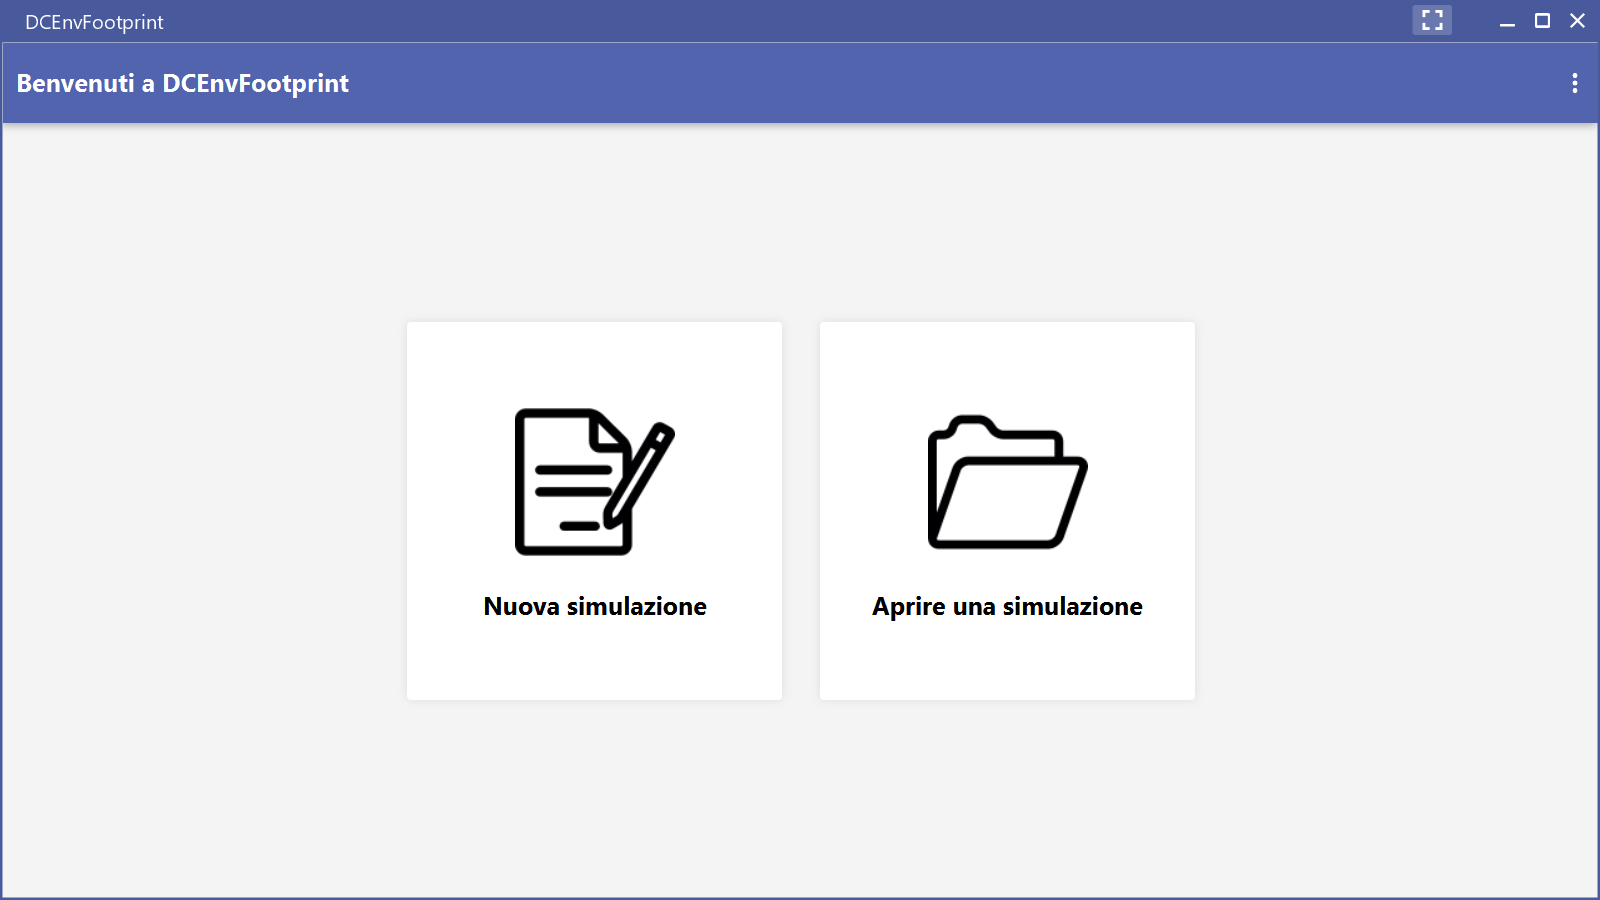
\includegraphics[scale=0.50]{partie2/images/italien.png}
		\caption{Le simulateur réglé en italien}
	\end{center}
\end{figure}
Le choix de la langue de l'utilisateur, qui se fait dans un menu en haut à droite, est sauvegardé. Pour ce faire nous utilisons un fonctionnalité de Java : les \code{Preferences}, qui permettent de stocker des couples clefs-valeurs très facilement sans se soucier du système d'exploitation. Ainsi lorsque l'utilisateur ferme et ré-ouvre le simulateur, la langue est reste inchangée. Ainsi le simulateur est disponible en anglais (plus ou moins exact) et en français.

\subsubsection{La réflexion autour de l'ergonomie}
Comme l'interaction avec les utilisateurs finaux à été quasiment inexistence, j'ai du pousser un peu plus loin la réflexion sur l'ergonomie que sur un projet plus classique où les retours réguliers des utilisateurs auraient permis de l'affiner. Le simulateur possède donc 2 menus, un menu latéral sur la gauche qui rappelle le nom de la simulation et affiche toutes les étapes de successives que l'utilisateur va suivre. L'utilisateur peut revenir à une étape qu'il a passé, mais ne peux pas aller sur les étapes grisés qui représente celles qu'il n'a pas encore remplis. J'ai également disposé un deuxième menu dans le coin supérieur droit qui permet d'effectuer des actions simples comme créer une nouvelle simulation, en ouvrir une existante, sauvegarde la simulation courante, changer les paramètres de  langues, afficher des informations générales sur le simulateur et quitter l'application.

\begin{figure}[h]
	\begin{center}
		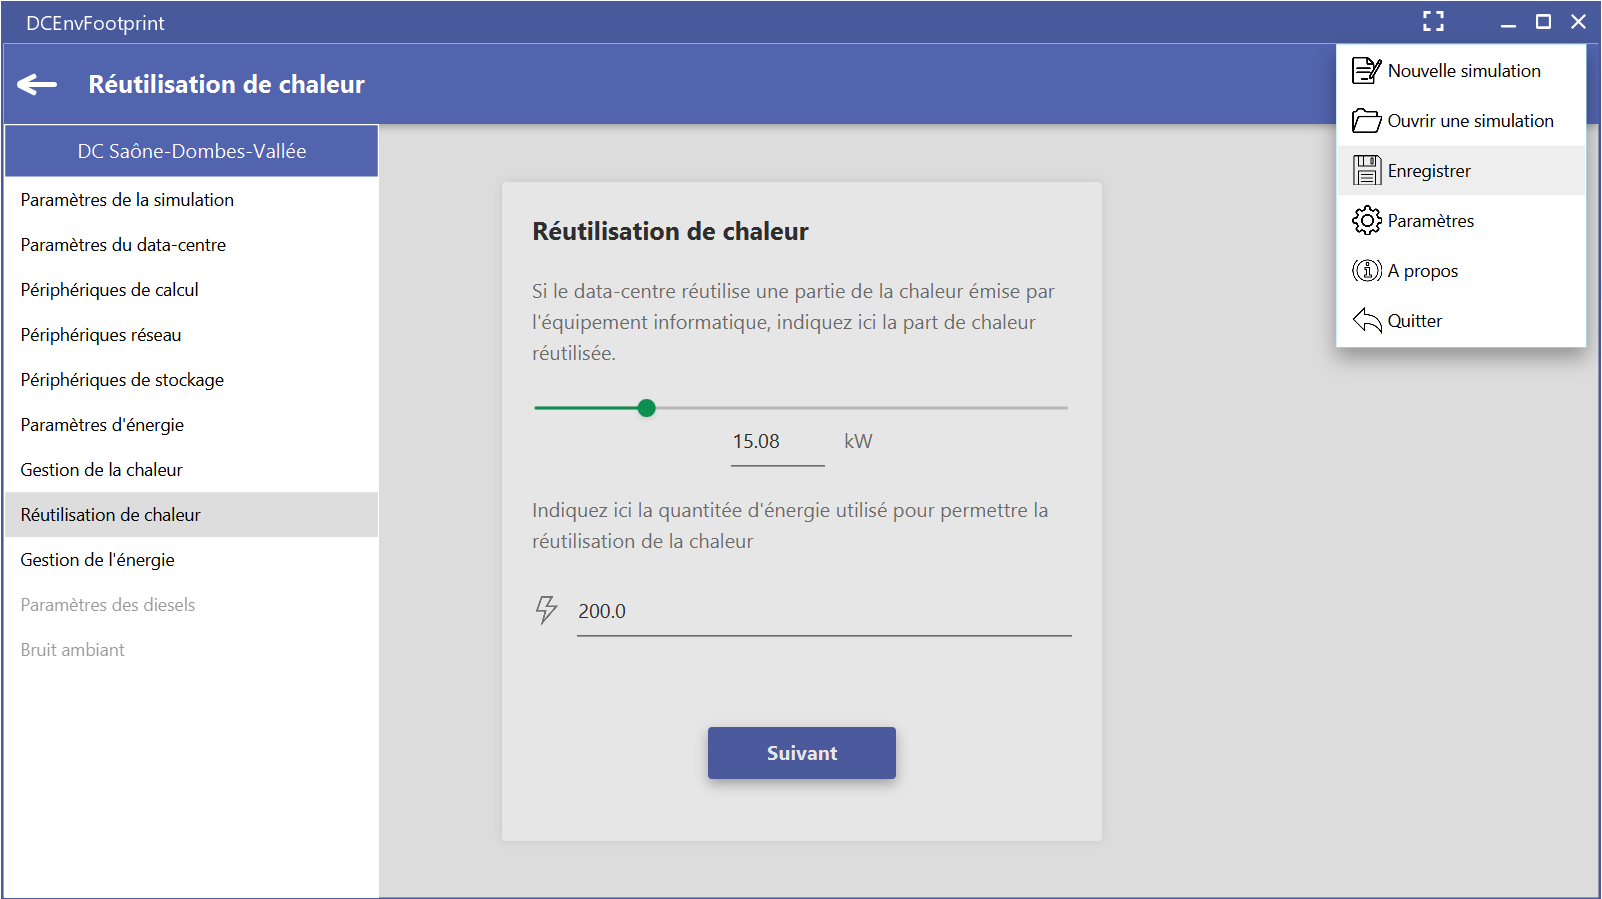
\includegraphics[scale=0.40]{partie2/images/ergonomie1.png}
		\caption{Les menus du simulateur}
	\end{center}
\end{figure}

Comme on peut le voir dans cet exemple, j'ai également fait le choix d'utiliser des composant d'interface graphique facile d'utilisation comme le slider tout en laissant à l'utilisateur le choix de précision avec un champs de texte qui est mis à jour et qui met à jour la valeur du slider ce qui permet un bon compromis.

\subsubsection{Les éléments d'interface personnalisés}
\begin{figure}[h!]
	\begin{minipage}{0.48\textwidth}
		\centering
		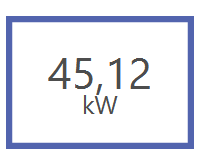
\includegraphics[height=4cm]{partie2/images/customcontrol1.png}
		\caption{Un indicateur de valeur avec unité}
	\end{minipage}\hfill
	\begin{minipage}{0.48\textwidth}
		\centering
		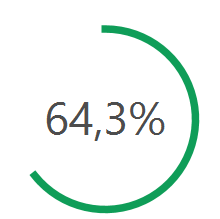
\includegraphics[height=4cm]{partie2/images/customcontrol2.png}
		\caption{Un indicateur de pourcentage}
	\end{minipage}\hfill
\end{figure}

Afin de coller au mieux a ce que j'imaginais pour l'affichage de certains indicateur, j'ai dû personnaliser certains éléments d'interface. J'ai réécris des partie du code source d'éléments graphiques déjà implémenté dans JavaFX ou dans JFoenix et je les ai modifié pour que je puisse les utiliser par la suite. Ainsi j'ai créé un indicateur de valeur avec une unité personnalisable, qui affiche automatique le bon ordre de grandeur de la valeur stocké : si 1000 W sont stocké  l'indicateur affichera 1 kW. J'ai également créé cette afficheur de pourcentage qui est basé sur un élément graphique représentant un temps de chargement.\\

J'ai également modifié le comportement d'une bonne partie d'éléments graphiques, sans les récréer complètement, afin qu'ils effectuent le comportement voulue. J'ai par exemple modifié les listes déroulante pour quelles affichent un icône, un titre et un description là où elle ne peuvent normalement n'afficher qu'un petit libellé. Pour ce faire j'ai réécris le code source des \code{Factory} de ces éléments. Une \code{Factory} est un module de code source qui crée applique à un élément son comportement, par exemple une \code{CellFactory} gère le comportement des cellules d'un tableau. La difficulté de cet exercie réside dans le fait qu'il faut s'insipirer du code source original pour espérer ne pas casser le fonctionnement de base de l'élément graphique. La librairie JFoenix est certes bien documenté, mais sa documentation ne possède pas un niveau de détail assez précis pour ce genre d'action, il est donc nécessaire faire appel à la connaissance de la communauté d'utilisateur de la librairie, notemment via des forums de discussion comme \emph{StackOverFlow}.

\subsubsection{La gestion des bases de données}
Pour certaines fonctionnalités le simulateur à besoins d'informations issues de base de données. C'est notamment le cas pour récupérer le poste électrique le plus proche dans le calcul de l'Indice d'Efficacité du Transport Electrique ou pour récupérer l'efficacité énergétique du matériel depuis la base de données \emph{SPEC}.\\
Ces données sont le plus souvent stockés dans des structures de données facilement lisible par l'humain, mais qui ne sont pas très performant pour leur exploitation automatique par un algorithme, comme par exemple les classeurs Excel. Pourtant le simulateur à besoin de faire des requêtes sur ces données pour extraire ce dont il a besoin.\\

Quoi de mieux pour faire des requêtes que d'utiliser le langage SQL que nous avons appris à l'IUT ? Afin d'exploiter les bases de données j'ai utilisé la technologie \emph{SQLite} qui est, comme son nom l'indique, une version légère de SQL. Son principal avantage est de pouvoir lire un base de données depuis un fichier directement sur la machine du client : donc pas besoin de serveur SQL pour répondre aux requêtes. De plus \emph{SQLite} propose un outils en ligne de commande qui permet de transformer les fichiers \code{.csv} en fichier \code{.sqlite}, j'ai donc pu convertir facilement les bases de données dans le bon format pour pouvoir les utiliser par la suite.

\subsubsection{Le calcul des indicateurs}
Le calcul des indicateurs est au centre du simulateur, c'est ce qu'il va permettre de générer le rapport et de d'évaluer les l'empreinte environnementale des centres de donnes. Ainsi tous les indicateurs sont codé \og en dure \fg{} dans le code source. Tous les indicateurs possèdent une architecture similaire. Chacun prend des paramètres d'entrées et génère un résultat qui est stocké afin de ne pas avoir à recalculer l'indicateur à chaque fois que l'on en a besoin. Toutes les étapes de calcul sont détaillés dans un dictionnaire associant une ligne de texte à une valeur afin de pouvoir retracer chaque étape du calcul de l'indicateur. Ainsi dans le rapport généré nous pouvons détailler assez précisément chaque étape de calcul. Les indicateurs possèdent également une source, sous forme d'adresse web, que l'on intégrera au rapport. L'utilisateur n'aura qu'a cliquer sur le lien pour avoir toutes les informations techniques relatives au calcul de l'indicateur.

\subsubsection{La génération du rapport}
Pour générer le rapport j'avais tout d'abord pensé à utiliser des outils de Business Intelligence puissants intégré en Java. Je pensais que l'utilisation de ces outils allaient me simplifier la tâche. C'était sans compter sur leur complexité et leurs concepts qui ne collaient pas totalement au résultat que je souhaitait avoir. J'ai notamment essayé la librairie \emph{JasperReport}, ce qui m'a fais perdre pas mal de temps.
J'ai alors complètement changé de méthode, en partant du principe que le plus simple serait le mieux.\\
J'utilise désormais un fichier HTML qui me sert de modèle, cela me permet de faire la mise en forme du rapport directement dans le fichier modèle et non pas lors de la génération. Ce fichier contient un éventail de mots clefs, facilement identifiables dans son code source. Pour générer le rapport il me suffit de lire le fichier modèle et de remplacer tous les mots clefs par des valeurs calculés.\\
J'ai distingué deux types de mots clefs. Tout d'abord les mots clefs de langue, entouré par des accolades (e.g.\ \code{\{SIMULATION\_AUTHORS\}}) qui correspondent à des entrées de textes présents dans les fichiers de langue. Ainsi le rapport peut être généré selon la langue choisie par l'auteur. Pour ce faire je recherche dans le fichier HTML toutes les entrées de langue présents dans le fichier de locale, et je les remplace par leur valeur associée. Le deuxième type de mots clefs sont les mots clefs de valeur (e.g\ \code{TOTAL\_SERVER\_AMOUNT}), non entouré d'accolade, ils sont remplacés au cas par cas par le simulateur selon ce qu'il doit être affiché.\\

Enfin, pour pouvoir générer un rapport au format PDF, j'enregistre sur le disque le modèle remplis avec les bonne valeur et j'utilise la librairie \emph{iText} qui me permet de convertir un fichier HTML en un fichier PDF.

\subsubsection{Créer un fichier exécutable}
Pendant toute la phase de développement, je lance le simulateur depuis mon \gls{ide} \gls{eclipse}. Cependant si je souhaite le distribuer il faut le compiler dans un fichier exécutable. Pour ce faire j'au utilisé la librairie \gls{maven} qui me permet de compiler tout le code source dans un seul fichier exécutable : le fichier \code{.jar}. Je pensais que cette phase allait se passer sans encombres, mai j'ai fais face à quelques problèmes.\\

Tout d'abord, pour charger mes ressources : images, fichiers vues ou fichiers de langues. Je recherchais dans le dossier sur le disque comprenant ses fichiers. Lorsque le simulateur est compilé en un seul fichiers, ces fichiers de ressources ne sont plus dans un dossier spécifique sur le disque mais dans un dossier compressé situé à l'intérieur du fichier compilé. Je ne peux donc pas accéder au ressources avec les moyens habituels. Pour palier à ce problème j'ai utilisé la lecture par flux : au lieu de lire un fichier physique, je lis un flux de données extrais du fichier \code{.jar}.\\

J'ai également fais face à un problème avec le chargement et la sauvegarde des simulation. Lorsque que je lançais le simulateur à partir du fichier exécutable compilé j'ai remarqué que certains caractères ne s'affichaient pas correctement. Pour régler ce problème j'ai forcer le simulateur à écrire et lire les fichiers de ressource dans un encodage spécifique : l'\emph{UTF-8}. Cet encodage est l'encodage le plus utilisé aujourd'hui et permet de coder la plupart des caractères utilisés dans le monde sans encombre. J'en ai déduis que l'environement dans lequel le simulateur était lancé depuis mon \gls{ide} avait comme encodage par défaut l'\emph{UTF-8}, alors que quand je lance le simulateur depuis le fichier exécutable l'encodage par défaut est celui du système d'exploitation (pour Windows il s'agit de l'\emph{ANSI}). Comme je n'avais pas donné de directive particulière pour l'encodage, le simulateur à simplement \og choisi \fg{} l'encodage par défaut.

\subsubsection{Faire face aux bugs des librairies}
Pour fonctionner le simulateur utilise 7 librairies tierces pour réaliser différentes fonctions. Ces librairies sont souvent le fruit d'un travail dans le cadre non professionnel par des développeur passionnés qui souhait ajouter leur pierre à l'édifice du logiciel libre. Ainsi certains librairies ne sont pas forcément maintenu régulièrement ou beaucoup testé avant leur mise en production. Fatalement ces librairies contiennent donc des bugs que le développeur qui les utilise ne pas corriger. Cela a été le cas avec le simulateur où j'ai par exemple découvert un bug de la librairie \emph{JFoenix} : les éléments graphique représentant un chargement (les \emph{spinner}) peuvent normalement rester fixe en se stopper à une valeur bien précise. Cependant lorsque l'on recharge l'écran, ce comportement disparait ! On se retrouve alors avec des \emph{spinner} qui tournent perpétuellement.\\

Afin que ce bug soit corriger dans le prochaine version de \emph{JFoenix}, j'ai créé un \gls{ticket} sur la page \gls{github} afin de signaler le bug. Les développeur de l'application y ont répondu et grâce à me contribution ce bug sera corrigé dans la prochaine version de \emph{JFoenix}.

\begin{figure}[h]
	\begin{center}
		\fbox{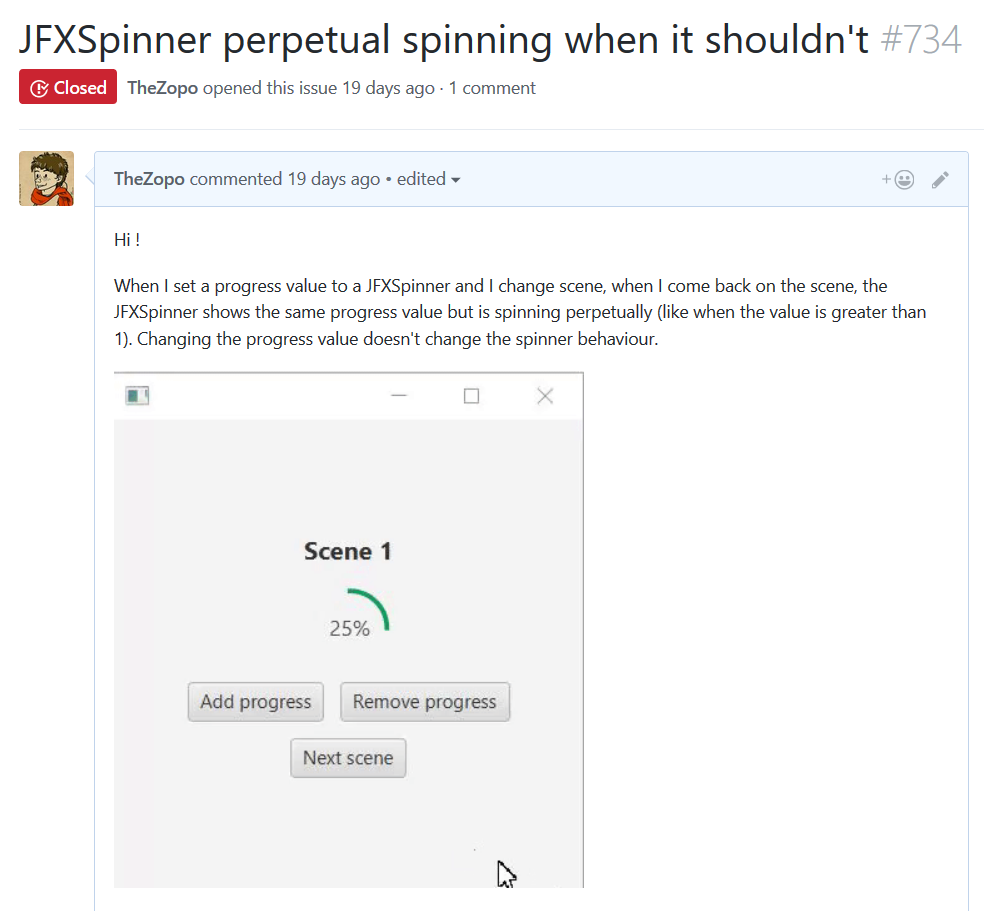
\includegraphics[scale=0.75]{partie2/images/ticket.png}}
		\caption{Une partie du ticket que j'ai créé sur la page de JFoenix}
	\end{center}
\end{figure}

